\documentclass[12pt,a4paper]{article}
\usepackage{amsmath}
\usepackage{amsfonts}
\usepackage{amssymb}
\usepackage{graphicx}
\usepackage{secdot}
\usepackage[left=2cm,right=2cm,top=2cm,bottom=2cm]{geometry}

\title{Experiment - 1\\Cyclic flow through a 90° bend}

\author{Arka Pramanick, AE21B007\\ Department of Aerospace Engineering\\ IIT Madras\\[3ex] Instructor:\\ \large Professor Dr. R. Sriram}

\date{05 February, 2023}


\begin{document}
\maketitle

\hline

\section{Aim :}
To examine the distribution of pressure in a cyclic flow using a 90° bend.
\section{Apparatus :}
Required apparatus for performing this experiment are:
\begin{itemize}
    \item A digital manometer (for measurement of pressure)
    \item A section of 90° bend with diameter 34 mm.
    \item A fan
\end{itemize}
\section{Theory :}
Pressure is more affected by the curvature ratio at the pipe's inner side than its outer side.When the gas elements move through the curved pipe,there are two accelerations : (i) one is $\frac{dw}{dt}$ along the tangential direction of the streamline and (ii) the another is the centripetal acceleration $\frac{\omega^2}{R}$ along the radius of curvature.The inertia forces are in equilibrium with pressure on the element and the following equations are obtained :
\begin{equation}
    -\frac{\partial p}{\partial n}+\rho \frac{\omega^2}{R} = 0\\
\end{equation}
\begin{equation}
    -\frac{\partial p}{\partial s}-\rho \frac{dw}{dt} = 0
\end{equation}
The Euler Equation in streamline co-ordinates with distance measured along streamline is $s$. Here, $s$ and $n$ being orthogonal to each other but the direction keeps changing.
As the flow along the streamline is considered, the velocity is always tangential to the streamline and hence there in no flow or velocity component along normal direction, i.e. $\Vec{u}= w\hat{i_s}$ . The radius of curvature R is defined as positive if $\hat{i_n}$ points away from the centre of curvature, and negative if $\hat{i_n}$ points toward it.
According to equation (1), we find that the pressure gradient along the -n direction is caused by centrifugal force due to fluid flow in the curved pipe.It is demonstrated that centrifugal force also affects the flow in the pipes upstream and downstream. Before the curved pipe enters, the pressure gradient initially drops and then climbs. The maximum pressure appears at $\theta=45^{\circ}$



\section{Procedure :}
\begin{enumerate}
    \item First fix the desired orifice(at $0^{\circ},45^{\circ}$ and $90^{\circ}$ across the bend of pipe for both inner and outer surface)  in the manometer.
    \item Gradually increase the speed of wind flowing inside after starting the machine.
    \item Take readings in all orifice for 3 different velocities.
\end{enumerate}






\section{Table and Graphs :}

\subsection{Negative Gauge Pressure for case 1 :}
 
\begin{center}
\begin{tabular}{ |c|c|c| } 
 \hline
 \textbf{$\theta$ in ($^{\circ}$)} & \textbf{Inner pressure (Pa)} & \textbf{Outer pressure (Pa)} \\ 
 \hline
0$^{\circ}$ & 1400 & 870 \\ 
 \hline
 45$^{\circ}$ & 1730 & 669 \\ 
 \hline
90$^{\circ}$ & 1400 & 850 \\ 
 \hline
\end{tabular}
\end{center}
\begin{figure}[!ht]
	\begin{center}
		\framebox{
			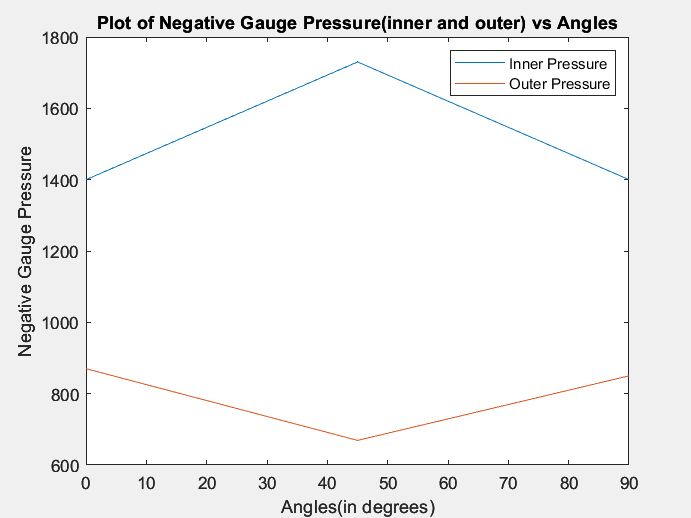
\includegraphics[scale=0.7]{lowspeed graph1 - Copy.png}
        }
	\end{center}
	\caption{Negative Gauge Pressure vs Angle for case 1}
\end{figure}
\newpage
\subsection{Negative Gauge Pressure for case 2 :}

\begin{center}
\begin{tabular}{ |c|c|c| } 
 \hline
 \textbf{$\theta$ in ($^{\circ}$)} & \textbf{Inner pressure (Pa)} & \textbf{Outer pressure (Pa)} \\ 
 \hline
0$^{\circ}$ & 2450 & 1460 \\ 
 \hline
 45$^{\circ}$ & 3000 & 1111 \\ 
 \hline
90$^{\circ}$ & 2350 & 1440 \\ 
 \hline
\end{tabular}
\end{center}
\begin{figure}[!ht]
	\begin{center}
		\framebox{
			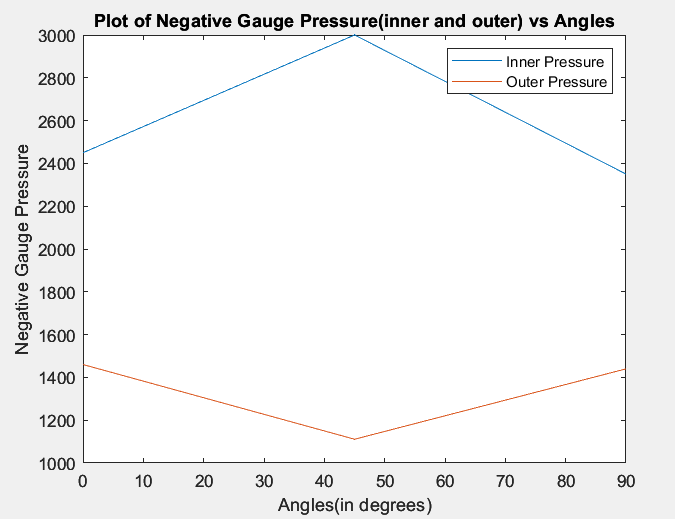
\includegraphics[scale=0.7]{lowspeed graph2.png}
		}
	\end{center}
	\caption{Negative Gauge Pressure vs Angle for case 2}
\end{figure}
\subsection{Negative Gauge Pressure for case 3 :}

\begin{center}
\begin{tabular}{ |c|c|c| } 
 \hline
 \textbf{$\theta$ in ($^{\circ}$)} & \textbf{Inner pressure (Pa)} & \textbf{Outer pressure (Pa)} \\ 
 \hline
0$^{\circ}$ & 1055 & 640 \\ 
 \hline
 45$^{\circ}$ & 1300 & 490 \\ 
 \hline
90$^{\circ}$ & 1040 & 640 \\ 
 \hline
\end{tabular}
\end{center}
\begin{figure}[!ht]
	\begin{center}
		\framebox{
			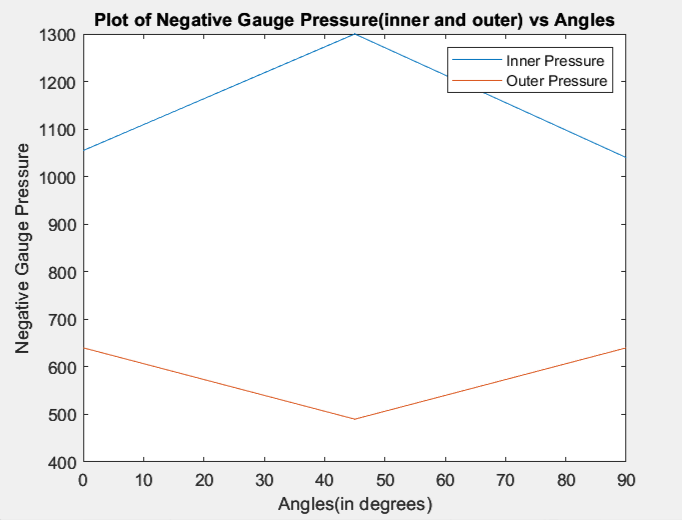
\includegraphics[scale=0.7]{lowspeed graph 3.png}
		}
	\end{center}
	\caption{Negative Gauge Pressure vs Angle for case 3}
\end{figure}
\newpage

\section{Sources of Error :}
\begin{itemize}
    \item Error in manometer.
    \item Error may cause while noting readings due to frequent changes in readings.
    \item Error may occur due to environmental effects like pressure difference,temperature difference etc.
\end{itemize}

\section{Conclusion :}

 The pressure difference in inner side decreases till 45°  and then it increases up to 90° but for outer side increases as the angle increases till 45° and then it decreases up to 90°. Since the velocity distribution is the characteristic distribution of a straight pipe,when it passes through the bend,it requires a centripetal acceleration in radially inwards direction to cross the bend.Due to which the fluid particles tends to move in radially outward direction to cross the bend. It leads to an decrease in pressure in the inner side of bend and increase in pressure in outer side of bend.
    

\end{document}